\chapter{QAbstractItemModel}

QAbstractItemModel类为项模型类提供了抽象接口。\href{https://github.com/JackLovel/QtDocumentCN/blob/master/Src/A/QAbstractItemModel}{更多...} 

\begin{tabular}{|r|l|}
	\hline
	属性 & 方法 \\
	\hline
	头文件 & \#include <QAbstractItemModel>\\      
	\hline
	qmake & QT+=core\\      
	\hline
	自从 & Qt 4.6\\
	\hline
	继承&QObject \\
	\hline
	派生 & \makecell{QAbstractListModel、QAbstractProxyModel、
           QAbstractTableModel、\\QConcatenateTablesProxyModel、QDirModel、QFileSystemModel \\和 QStandardItemModel} \\
	\hline
\end{tabular}

\splitLine

公有成员类型

\resizebox{\textwidth}{!}{
\begin{tabular}{|r|l|}
	\hline
	类型 & 类型名称 \\
	\hline
enum class&	CheckIndexOption{ NoOption, IndexIsValid,
  DoNotUseParent, ParentIsInvalid}\\
\hline
flags&	CheckIndexOptions\\
\hline
enum&	LayoutChangeHint { NoLayoutChangeHint, VerticalSortHint, HorizontalSortHint }\\
\hline
\end{tabular}}


\splitLine

公共成员函数

\begin{longtable}{|r|l|}
\hline
类型 & 函数名称 \\
\hline
& QAbstractItemModel(QObject *parent = nullptr)\\
\hline
virtual	& $\sim$QAbstractItemModel()\\
\hline
virtual QModelIndex	& buddy(const QModelIndex \&index) const\\
\hline
virtual bool & canDropMimeData(const QMimeData *data, Qt::DropAction
               action, int row, int column, const QModelIndex
               \&parent) const s\\
\hline
virtual bool &canFetchMore(const QModelIndex \&parent) const\\
\hline
bool & checkIndex(const QModelIndex \&index,
       QAbstractItemModel::CheckIndexOptions options =
       CheckIndexOption::NoOption) const\\
\hline
virtual int&columnCount(const QModelIndex \&parent = QModelIndex())
             const = 0\\
\hline
virtual QVariant&	data(const QModelIndex \&index, int role = Qt::DisplayRole) const = 0\\
\hline
virtual bool&	dropMimeData(const QMimeData *data, Qt::DropAction
              action, int row, int column, const QModelIndex \&parent)\\
\hline
virtual void&	fetchMore(const QModelIndex \&parent)\\
\hline
virtual Qt::ItemFlags&	flags(const QModelIndex \&index) const\\
\hline
virtual bool&	hasChildren QModelIndex \&parent = QModelIndex()) const\\
\hline
bool	&hasIndex row, int column, const QModelIndex \&parent = QModelIndex()) const\\
\hline
virtual QVariant	&headerData section, Qt::Orientation orientation, int role = Qt::DisplayRole) const\\
\hline
virtual QModelIndex& index row, int column, const QModelIndex \&parent = QModelIndex()) const = 0\\
\hline
bool	&insertColumn column, const QModelIndex \&parent = QModelIndex())\\
\hline
virtual bool & insertColumns column, int count, const QModelIndex \&parent = QModelIndex())\\
\hline
bool&	insertRow(int row, const QModelIndex \&parent = QModelIndex())\\
\hline
virtual bool&	insertRows row, int count, const QModelIndex \&parent
              = QModelIndex())\\
\hline
virtual QMap<int, QVariant>	&itemData QModelIndex \&index) const\\
\hline
virtual QModelIndexList	& match QModelIndex \&start, int role, const QVariant \&value, int hits = 1, Qt::MatchFlags flags = Qt::MatchFlags (Qt::MatchStartsWith\\
\hline
virtual QMimeData *	&mimeData QModelIndexList \&indexes) const\\
\hline
virtual QStringList	& mimeTypes const\\
\hline
bool	&moveColumn QModelIndex \&sourceParent, int sourceColumn,
       const QModelIndex \&destinationParent, int destinationChild)\\
\hline
virtual bool & moveColumns QModelIndex \&sourceParent, int
               sourceColumn, int count, const QModelIndex
               \&destinationParent, int destinationChild)\\
\hline
bool& moveRow QModelIndex \&sourceParent, int sourceRow, const QModelIndex \&destinationParent, int d
estinationChild)\\
\hline
virtual bool &moveRows QModelIndex \&sourceParent, int sourceRow, int destinationChild)\\
\hline
bool &moveRow QModelIndex \&sourceParent, int sourceRow, 
       const QModelIndex \&destinationParent, 
       int destinationChild)\\    
\hline           
virtual bool &moveRows QModelIndex \&sourceParent, int sourceRow, 
               int count, const QModelIndex \&destinationParent, int destinationChild)\\
\hline
virtual QModelIndex&	parent QModelIndex \&index) const = 0\\
\hline
bool&	removeColumn column, const QModelIndex \&parent = QModelIndex())\\
\hline
virtual bool&	removeColumns column, int count, const QModelIndex \&parent = QModelIndex())\\
\hline
bool&	removeRow row, const QModelIndex \&parent = QModelIndex())\\
\hline
virtual bool&	removeRows row, int count, const QModelIndex \&parent = QModelIndex())\\
\hline
virtual QHash<int, QByteArray>&	roleNames const\\
\hline
virtual int	& rowCount QModelIndex \&parent = QModelIndex()) const = 0\\
\hline
virtual bool &setData QModelIndex \&index, const QVariant \&value, int role = Qt::EditRole)\\
\hline
virtual bool	&setHeaderData section, Qt::Orientation orientation, const QVariant \&value, int role = Qt::EditRole)\\
\hline
virtual bool	&setItemData QModelIndex \&index, const QMap<int, QVariant> \&roles)\\
\hline
virtual QModelIndex&	sibling row, int column, const QModelIndex \&index) const\\
\hline
virtual void	&sort column, Qt::SortOrder order = Qt::AscendingOrder)\\
\hline
virtual QSize	&span QModelIndex \&index) const\\
\hline
virtual Qt::DropActions	&supportedDragActions const\\
\hline
virtual Qt::DropActions	&supportedDropActions const\\
\hline
\end{longtable}

\splitLine

公共槽函数

\begin{tabular}{|r|l|}
\hline
类型 & 函数名称 \\
\hline
virtual void	&revert()\\
\hline
virtual bool	&submit()\\
\hline
\end{tabular}

\splitLine

信号

\resizebox{\textwidth}{!}{
\begin{tabular}{|r|l|}
\hline
类型 & 函数名称 \\
\hline
void&	columnsAboutToBeInserted QModelIndex \&parent, int first, int last)\\
\hline
void&	columnsAboutToBeMoved(const QModelIndex \&sourceParent, int sourceStart, int sourceEnd, const QModelIndex \&destinationParent, int destinationColumn)\\
\hline
void&	columnsAboutToBeRemoved(const QModelIndex \&parent, int first, int last)\\
\hline
void&	columnsInserted(QModelIndex \&parent, int first, int last)\\
\hline
void&	columnsMoved(const QModelIndex \&parent, int start, int end, const QModelIndex \&destination, int column)\\
\hline
void&	columnsRemoved(const QModelIndex \&parent, int first, int last)\\
\hline
void&	dataChanged(const QModelIndex \&topLeft, const QModelIndex \&bottomRight, const QVector \&roles = QVector())\\
\hline
void&	headerDataChanged(Qt::Orientation orientation, int first, int last)\\
\hline
void&	layoutAboutToBeChanged(const QList \&parents = QList(), QAbstractItemModel::LayoutChangeHint hint = QAbstractItemModel::NoLayoutChangeHint)\\
\hline
void&	layoutChanged(const QList \&parents = QList(),
      QAbstractItemModel::LayoutChangeHint hint = QA
bstractItemModel::NoLayoutChangeHint)\\
\hline
void&	modelAboutToBeReset()\\
\hline
void&	modelReset()\\
\hline
void&	rowsAboutToBeInserted(const QModelIndex \&parent, int start, int end)\\
\hline
void&	rowsAboutToBeMoved(const QModelInd
ex \&sourceParent, int
      sourceStart, int sourceEnd, const QM
odelIndex \&destinationParent, int destinationRow)\\
\hline
void&	rowsAboutToBeRemoved(const QModelIndex \&parent, int first, int last)\\
\hline
void&	rowsInserted(const QModelIndex \&parent, int first, int last)\\
\hline
void&rowsMoved(const QModelIndex \&parent, int start, 
  int end, const QModelIndex \&destination, int row) \\
\hline
void&	rowsRemoved(const QModelIndex \&parent, int first, int last)\\
\hline
\end{tabular}}

\splitLine

受保护的函数

\resizebox{\textwidth}{!}{
\begin{tabular}{|r|l|}
\hline
类型 &	 函数名称\\
\hline
void&	beginInsertColumns(const QModelIndex \&parent, int first, int
      last)\\
\hline
void&	beginInsertRows(const QModelIndex \&parent, int first, int
      last)\\
\hline
bool&	beginMoveColumns(const QModelIndex \&sourceParent, int
  sourceFirst, int sourceLast, const QModelIndex \&destinationParent,
  int destinationChild)\\
\hline
bool&	beginMoveRows(const QModelIndex \&sourceParent, int
      sourceFirst, int sourceLast, const QModelIndex
      \&destinationParent, int destinationChild)\\
\hline
void&	beginRemoveColumns(const QModelIndex \&parent, int first, int
      last)\\
\hline
void&	beginRemoveRows(const QModelIndex \&parent, int first, int last)\\
\hline
void&	beginResetModel()\\
\hline
void&	changePersistentIndex(const QModelIndex \&from, const QModelIndex \&to)\\
\hline
void&	changePersistentIndexList(const QModelIndexList \&from, const
   QModelIndexList \&to)\\
\hline
QModelIndex&	createIndex(int row, int column, void *ptr = nullptr) const\\
\hline
QModelIndex&	createIndex(int row, int column, quintptr id) const\\
\hline
void&	endInsertColumns()\\
\hline
void&	endInsertRows()\\
\hline
void&	endMoveColumns()\\
\hline
void&	endMoveRows()\\
\hline
void&	endRemoveColumns()\\
\hline
void&	endRemoveRows()\\
\hline
void&	endResetModel()\\
\hline
QModelIndexList&	persistentIndexList() const\\
\hline
\end{tabular}}

受保护的槽函数

\splitLine

\begin{tabular}{|r|l|}
\hline
类型 	&函数名称\\
\hline
void	&resetInternalData()\\
\hline
\end{tabular}

详细描述

\splitLine

QAbstractItemModel 类定义了项模型与模型/视图体系结构中的其他组件进行交互操作时必须使用的标准接口。应该子类化该类创建新的模型,而不是直接实例化使用。

QAbstractItemModel 类是模型/视图类中的一个,也是 Qt 模型/视图框架的一部分。它可以用作 QML 中的项视图元素或 Qt Widgets 模块中的项视图类的底层数据模型。

如果需要一个模型来使用项视图,比如 QML 的 List View 元素或者 C++ widgets 的 QListView 或者  QTableView,应该考虑子类化 QAbstractListModel 或者 QAbstractTableModel 而不是使用该类。

底层数据模型作为表的层次结构暴露给视图和委托。如果不使用层次结构,那么模型就是一个简单的具有行和列的表。每个项都有一个由 QModelIndex 指定的惟一索引。

\begin{figure}[hbt!]  
	\centering
    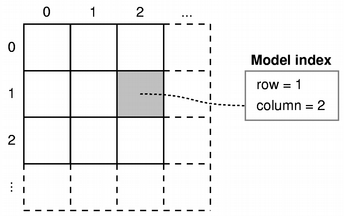
\includegraphics[width=0.5\textwidth]{modelindex-no-parent}
	\caption{model index}
\end{figure}

每个数据项都可以通过包含一个关联的模型索引的模型进行访问。该索引可以通过 index() 函数获得。每个索引可能有一个 sibling() 索引;子项有一个 parent() 索引。

每个项目都有许多与之关联的数据元素,可以通过为模型的 data() 函数指定一个角色(请参阅 Qt::ItemDataRole)来检索它们。可以使用 itemData() 函数同时获取所有可用角色的数据。

使用特定的 Qt::ItemDataRole 设置每个角色的数据。可以使用 setData() 单独设置各个角色的数据,也可以使用 setItemData 设置所有角色的数据。

可以使用 flags() 查询项(请参阅 Qt::ItemFlag),以查看是否可以通过其他方式选择,拖动或操纵它们。

如果项具有子对象,则 hasChildren 为相应的索引返回 true。

该模型在层次结构的每个级别都有一个 rowCount() 和 columnCount。可以使用 insertRows(),insertColumns(),removeRows() 和 removeColumns() 插入和删除行和列。

模型发出信号以指示变化。例如,只要模型可用的数据项发生更改,就会发出 dataChanged()。对模型提供的标题的更改将将发射 headerDataChanged() 信号。如果底层数据的结构发生了变化,则模型可以发出 layoutChanged() 来向任何附加的视图指示它们应该重新显示所显示的任何项,并需要考虑到新的结构。

可以使用 match() 函数在模型中搜索可用的项以查找特定数据。

要对模型进行排序,可以使用 sort()。

\splitLine

子类化

注意: 在模型子类化参考中有一些关于模型子类化的通用指南。

子类化 QAbstractItemModel 时,至少必须实现 index(),parent(),rowCount(),columnCount() 和 data()。这些函数在所有的只读模型中使用,同样也构成了可编辑模型的基础。

还可以为模型重新实现 hasChildren() 来提供特殊的行为,而不是重新实现成本很高的 rowCount()。这使得模型可以限制视图请求的数据量,并且可以作为实现模型数据的惰性填充的一种方式。

要在模型中启用编辑,还必须实现 setData 和重新实现 flags() 以确保返回 ItemIsEditable。还可以重新实现 headerData() 和 setHeaderData 来控制呈现模型标题的方式。

当分别重新实现 setData() 和 setHeaderData() 函数时,必须显式发射 dataChanged() 和 headerDataChanged() 信号。

定制模型需要创建模型索引以供其他组件使用。为此,请使用适当的行号和列号以及相应的标识符调用 createIndex(),并将其作为指针或整数值。这些值的组合对于每个项都必须是唯一的。定制模型通常在其他重新实现的函数中使用这些唯一标识符,以检索项数据并访问有关该项的父项和子项的信息。有关唯一标识符的更多信息,请参见简单树模型示例。

不必支持 Qt::ItemDataRole 中定义的每个角色。根据模型中包含的数据类型,可能只有实现 data() 函数以返回一些更常见角色的有效信息才有用。大多数模型至少为 Qt::DisplayRole 提供项数据的文本表示,行为良好的模型也应为 Qt::ToolTipRole 和 Qt::WhatsThisRole 提供有效信息。支持这些角色可使模型与标准 Qt 视图一起使用。但是,对于某些处理高度专业化数据的模型,仅为用户定义的角色提供数据可能是合适的。

提供可调整数据结构大小的接口的模型可以提供 insertRows(),removeRows(),
insertColumns() 和 removeColumns() 的实现。在实现这些函数时,重要的是
要在模型尺寸大小发生 之前 和 之后 将有关模型尺寸的更改通知所有连接的视
图:

\begin{itemize}
\item insertRows() 的实现必须在将新行插入数据结构 之前 调用
  beginInsertRows(),然后立即 调用 endInsertRows()。
\item insertColumns() 的实现必须在将新列插入数据结构 之前 调用
  beginInsertColumns(),然后立即 调用 endInsertColumns()。
\item removeRows() 的实现必须在从数据结构中删除行 之前 调用
  beginRemoveRows(),然后立即 调用 endRemoveRows()。
\item removeColumns() 的实现必须在列从数据结构中删除之前调用 beginRemoveColumns(),然后立即 调用 endRemoveColumns()。
\end{itemize}

这些函数发出的私有信号使附加组件有机会在任何数据变得不可用之前采取行动。使用这些 begin 和 end 函数封装插入和删除操作还使模型能够正确地管理持久模型索引。如果希望正确处理选择,则必须确保调用了这些函数。 如果插入或移除带有子项的项,则不需要为子项调用这些函数。换句话说,父项将管理其子项。

要创建增量填充的模型,可以重新实现 fetchMore() 和 canFetchMore()。如果 fetchMore() 的重新实现向模型中添加了行,则必须调用 beginInsertRows() 和 endInsertRows()。

参见模型类、模型子类化参考、QModelIndex、QAbstractItemView、在项视图中
使用拖放、简单DOM模型示例、简单树模型示例、可编辑树模型示例和 Fetch
More示例。

\splitLine

成员类型文档

CheckIndexOption CheckIndexOptions
enum class QAbstractItemModel::CheckIndexOption flags QAbstractItemModel::CheckIndexOptions

这个枚举可以用来控制 QAbstractItemModel::checkIndex() 执行的检查。

\resizebox{\textwidth}{!}{ % 文本过宽
\begin{tabular}{|l|l|l|}
\hline
常量 &值&描述\\
\hline
QAbstractItemModel::CheckIndexOption::NoOption & 0x0000	& 没有指定检查选项。\\
\hline
QAbstractItemModel::CheckIndexOption::IndexIsValid&0x0001&传递给 QAbstractItemModel::checkIndex()的模型索引被检查为有效的模型索引。\\
\hline
QAbstractItemModel::CheckIndexOption::DoNotUseParent&0x0002&不执行任何涉及到传递给 QAbstractItemModel::checkIndex() 的父索引的使用的检查。\\
\hline
\end{tabular}}

该枚举是在 Qt 5.11 中引入或修改的。

CheckIndexOptions 类型是一个 QFlags<CheckIndexOption> 的类型定义。它存储一个或组合的 CheckIndexOption 值。

\splitLine

LayoutChangeHint

enum QAbstractItemModel::LayoutChangeHint

这个枚举描述了模型改变布局的方式。

\begin{tabular}{|l|l|l|}
\hline
常量 &值&描述\\
\hline
QAbstractItemModel::NoLayoutChangeHint&	0&	没有任何提示。\\
\hline
QAbstractItemModel::VerticalSortHint&	1&	正在对行进行排序。\\
\hline
QAbstractItemModel::HorizontalSortHint&	2&	正在对列进行排序。\\
\hline
\end{tabular}

注意,VerticalSortHint 和 HorizontalSortHint 表示项在同一父级中移动,
而不是移动到模型中的不同父级,也没有过滤掉或过滤进来。

\splitLine

成员函数文档

QAbstractItemModel

QAbstractItemModel::QAbstractItemModel(QObject *parent = nullptr)

构造指定父类对象 parent 的抽象项模型。

columnsAboutToBeInserted
[signal] void QAbstractItemModel::columnsAboutToBeInserted(const QModelIndex \&parent, int first, int last)

在将列插入模型之前就发射此信号。新项将位于给定父项 parent 下的首 first 尾 last之间。

注意: 连接到这个信号的组件使用它来适应模型尺寸的变化。它只能由 QAbstractItemModel 的实现发射,不能在子类代码中显式发射。

注意: 这是一个私有信号。它可以用于信号连接,但不能由用户发射。

参见 insertColumns() 和 beginInsertColumns()。
%%% Local Variables:
%%% mode: latex
%%% TeX-master: "../../master"
%%% End:
